In the scope of simplifying the configuration of a given product line some specific tools and techniques were used. This section will give an overview of what was used in this work to archive the simplification.

\subsection{Feature Models}
Feature models are multi-purpose structure for product lines. 
\begin{figure}
	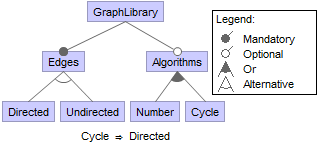
\includegraphics{img/img-fm.png}
	\caption{A simple example of a feature model}
	\label{img-fm}
\end{figure}
Amongst their benefits are:
\begin{itemize}
\item Can be visualized as a feature diagram, showing the possible features and their hierarchy
\item Classification of features and their dependencies (alternative/or; optional/mandatory/abstract)
\item Formal Representation of the whole product line as a feature diagram $\Rightarrow$ computationally processable
\item Enables configuration and variant validation
\end{itemize}
Although feature models can be represented as a boolean formula in CNF or grammer (GUIDSL), it is typically represented in form of a feature diagram and constraints. The feature diagram is basically structured as a tree: There is a root node, an arbitrary number of levels of nodes and finally leaf nodes without child nodes of their own. In that manner feature models map the hierarchy of features. Non-leaf features are often marked as abstract, as they do not have to be implemented. In addition features can be marked as either mandatory or optional. The possible relationships of multiple features with a mutual parent feature are \textit{OR} (at least one feature has to be selected), \textit{ALTERNATIVE} (exactly one feature has to be selected) and \textit{AND} (any number of features can be selected). As features' relations may be of higher complexity than just parent-child relations additional constraints can be noted within a feature model. Constraints can contain any boolean expression.

Figure~\ref{img-fm} shows an example of a simple feature model diagram. The node labeled "GraphLibrary" is the root feature and represents the whole Project. It contains the nodes "Edges" that has to be selected doe to the mandatory marker and "Algorithms" that is marked optional. The implemented Edge types are "Directed" and "Undirected" from which exactly one has to be chosen. From the Algorithms at least one has to be chosen. The Constraint beneath the figure~\ref{img-fm} implies that if the feature "Cycle" is selected, the Edge type is set to directed.

\subsection{Product configuration}
The whole product line is represented by it's feature model, which itself is a set of features with specific interrelations. The process of configuration of a product line describes the steps to derive a product from the product line. To archive this, one has to select a subset of all the possible features within the product line to meet one's requirements. But not all subsets of features result in an actual product. The interrelations of the features restrict the possible combinations of features resulting in a \textit{valid} configuration. If only one of the requirements from the interrelations between the features is not met, no product can be created and the configuration as such is considered \textit{invalid}.

During configuration a user selects or unselects features to his needs. This process requires a lot of domain knowledge on the one hand and detailed information about each single feature on the other. With growing numbers of possible features (and thus growing numbers of possible products) configuration requires more and more effort. The sheer amount of time needed to iterate over all the features grows to be significant. But the even greater problem arises from the possible interactions and interrelations of features, which one has to keep track of during configuration. The overhead of configuration might even outright negate the benefit gained from using a product line instead of multiple stand-alone products.

{\color{red}TODO: introduce partial configuration}

\subsection{Constraints, contradictions, SAT-solver}
A feature-tree (from a feature model) can be expressed as a boolean statement. The mapping between the individual groups (sub-trees) and the corresponding boolean expression is shown in the folloing list:

{\color{red}TODO: Rules for
\begin{itemize}
	\item Or
	\item Alternative
	\item And
\end{itemize}
}
These particular groups are joined via a boolean \textit{AND}. For the example feature tree shown in figure~\ref{img-fm} the corresponding boolean expression is as follows:
\begin{equation}
\begin{split}
	GraphLibrary\ \wedge\ Edges\\
	\wedge\ ((Directed\ \wedge \neg Undirected)\\
	\vee (\neg Directed\ \wedge\ Undirected))
\end{split}
\end{equation}\\

As the feature model not only contains the feature tree, but also additional constraints, these constraints have to be considered in the boolean expression representing the complete feature model. They can be linked to one another via boolean \textit{AND}s. The connection to the previously created boolean expression of the feature tree is also made through a logical \textit{AND}. Thus, the complete resulting boolean expression for the feature model shown in figure~\ref{img-fm} is:
\begin{equation}
\begin{split}
	GraphLibrary\ \wedge\ Edges\\
	\wedge\ ((Directed\ \wedge \neg Undirected)\\
	\vee (\neg Directed\ \wedge\ Undirected))\\
	\wedge\ (Algorithms\ \Rightarrow\ (Number\ \vee\ Cycle))\\
	\wedge\ (Cycle\ \Rightarrow\ Directed)
\end{split}
\end{equation}\\
This formalism allows a configuration to be checked for validity. To do so each selected Feature is appended with a logical \textit{AND} and each specifically unselected feature is also appended with a logical \textit{AND} but gets negated. The resulting expression is then evaluated by a SAT-solver to check for satisfiability. Even during configuration this process can be applied to check for invalid partial configurations after each decision.
